\chapter{The Method of Characteristics}
\label{chap:moc}

In the previous chapter, some significant approximations are made in generation of multi-group cross-sections. Standard \ac{MOC} solvers, such as the one developed and discussed in this thesis, rely on multi-group cross-sections as input. Once the cross-sections are generated, \ac{MOC} is capable of computing reaction rates across the reactor geometry.

First, the \ac{MOC} equations are derived from the multi-group neutron transport equation. Then, track discretization is introduced, forming a system of equations involving discrete variables. Finally, the solution of the system of equations is discussed. Discussions of solution techniques to the \ac{MOC} system of equations normally are centered around the underlying physics with little mention of the system as a linear algebra problem~\cite{boyd2014openmoc}. Others further describe \ac{MOC} in terms of operator notation, but offer little insight into the structure of the operators~\cite{kochunas}. Instead, this discussion casts the system of equations as simply a general eigenvalue problem. Then discussion of matrix structure motivates the use of an uncommon solution technique. Physical reasoning for the structure is mentioned throughout the discussion. The properties of the chosen solution technique are discussed, motivating the need for an acceleration scheme to mitigate its weaknesses.


%%%%%%%%%%%%%%%%%%%%%%%%%%%%%%%%%%%%%%%%%%%%%%%%%%%%%%%%%%%%%%%%%%%%%%%%%%%%%%%
\section{Derivation of Continuous Angle MOC Equations}
\label{sec:derivation-of-moc}

Starting from the multi-group neutron transport equation given in Eq.~\ref{eqn:multi-group-transport}, the neutron source $q_g(\mathbf{r})$ is defined in Eq.~\ref{eqn:source},
\begin{equation}
q_g(\mathbf{r}) = \frac{1}{4 \pi} \left( \frac{\chi_{g}\left(\mathbf{r}\right)}{k} \sum_{g'=1}^{G} \nu_{g'}\left(\mathbf{r}\right) \Sigma_f^{g'}\left(\mathbf{r}\right) \phi_{g'}\left(\mathbf{r}\right) + \, \sum_{g'=1}^G \,  \Sigma_{s}^{g' \rightarrow g}\left(\mathbf{r}\right) \phi_{g'}(\mathbf{r}) \right)
\label{eqn:source}
\end{equation}
which leads to a new form for the neutron balance equation in Eq.~\ref{eqn:source-balance}.
\begin{dmath}
	\mathbf{\Omega} \cdot \nabla \psi_g(\mathbf{r},\mathbf{\Omega}) \, + \, \Sigma_{t}^{g}(\mathbf{r})\psi_g(\mathbf{r},\mathbf{\Omega}) = q_g(\mathbf{r})
	\label{eqn:source-balance}
\end{dmath}
Next, a coordinate transformation is performed, casting the position as a displacement from an origin $\mathbf{r_0}$ along the direction of travel $\mathbf{\Omega}$ as $\mathbf{r} = \mathbf{r_0} + s\mathbf{\Omega}$. Under this transformation, the new balance equation becomes:
\begin{dmath}
	\mathbf{\Omega} \cdot \nabla \psi_g(\mathbf{r_0} + s\mathbf{\Omega},\mathbf{\Omega}) \, + \, \Sigma_{t}^{i,g}(\mathbf{r_0} + s\mathbf{\Omega})\psi_g(\mathbf{r_0} + s\mathbf{\Omega},\mathbf{\Omega}) = q_g(\mathbf{r_0} + s\mathbf{\Omega})
\end{dmath}
In this new form, the gradient reduces to a simple derivative by the distance $s$ traveled from the origin $\mathbf{r_0}$ in Eq.~\ref{eqn:moc-transform}.
\begin{dmath}
	\frac{d\psi_g(\mathbf{r_0} + s\mathbf{\Omega},\mathbf{\Omega})}{ds} \, + \, \Sigma_{t}^{g}(\mathbf{r_0} + s\mathbf{\Omega})\psi(\mathbf{r_0} + s\mathbf{\Omega},\mathbf{\Omega}) = q_g(\mathbf{r_0} + s\mathbf{\Omega})
	\label{eqn:moc-transform}
\end{dmath}
Considering a region $i$ with constant total cross-section $\Sigma_{t}^{i,g}$, the angular flux a distance $\ell$ from the origin can be calculated using Eq.~\ref{eqn:moc-source-int}. The interested reader can find a simple derivation in Appendix~\ref{deriv:moc-source-int}.
\begin{dmath}
	\psi_g(\mathbf{r_0} + \ell \mathbf{\Omega},\mathbf{\Omega}) = \psi_g(\mathbf{r_0},\mathbf{\Omega}) e^{-\Sigma_{t}^{i,g} \ell} + \int\displaylimits_{0}^{\ell} ds \, e^{-\Sigma_{t}^{i,g} (\ell-s)}q_g(\mathbf{r_0} + s\mathbf{\Omega})
	\label{eqn:moc-source-int}
\end{dmath}

Eq.~\ref{eqn:moc-source-int} reveals an important relationship. For a region of constant total cross-section with known source distribution $q_g(\mathbf{r})$ and angular flux at a single point $\psi_g(\mathbf{r_0},\mathbf{\Omega})$, the angular flux for all points along the direction of travel $\mathbf{\Omega}$ can be calculated. Therefore an enclosing boundary defining the relationship of impinging angular fluxes is sufficient for the calculation of all angular fluxes within the region.

An example of one such boundary condition is the vacuum boundary condition where it is assumed that zero angular flux is impingent on the region for all angles. This is often used for full core problems since there are virtually no neutron sources outside the problem domain.

If the problem domain can be represented (or approximated) as the composition of a finite number of \textit{source regions} over which the total cross-section is constant and the neutron source $q_g(\mathbf{r})$ takes some known distribution, the calculation of all angular fluxes throughout the problem is straightforward.

Realistically, the source distribution is not known before solving the neutron transport equation, since it depends on the scalar fluxes. However, if the geometry is sufficiently discretized, a low order approximation of the \textit{shape} of the neutron source within the regions can be made with little impact on solution accuracy. An example of geometry discretization is shown in Fig.~\ref{fig:pin-discretization} where a fuel pin is discretized radially. The image on the left shows a radial view of the fuel pin geometry, colored by (constant cross-section) material region. The image on the right shows a discretized form of that geometry, colored by source region over which the neutron source is assumed to have some low-order form.

\begin{figure}[h!]
	\centering
	\begin{subfigure}{0.45\textwidth}
		\centering
		
\includegraphics[width=\linewidth]{figures/pin_1.PNG}
		\caption{}
		\label{fig:pin-discretization-a}
	\end{subfigure}
	\begin{subfigure}{0.45\textwidth}
		\centering
		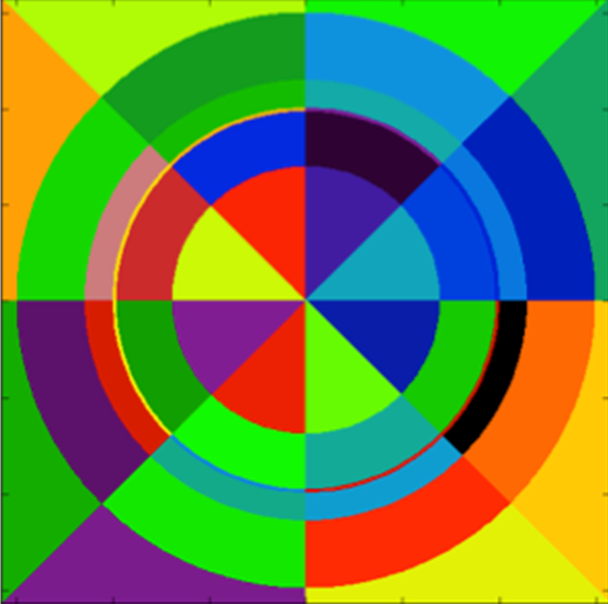
\includegraphics[width=\linewidth]{figures/pin_1_discretized.PNG}
		\caption{}
		\label{fig:pin-discretization-b}
	\end{subfigure}
	\caption[]{A description of source region discretization and mesh refinement. The geometry is shown (a) colored by material and (b) colored by source region.}
	\label{fig:pin-discretization}
\end{figure}

One common low order approximation for the neutron source is the flat source approximation. This approximation assumes the neutron source for a given energy group $q_g(\mathbf{r})$ is constant over each source region. A linear source approximation will be introduced later in Section~\ref{sec:linear-source}, allowing for a coarser discretization of the geometry. However, the flat source approximation is first presented in this description of \ac{MOC} as it is less mathematically cumbersome than the linear source approximation while arriving at a very similar form and solution method as the linear source version. The flat source approximation is also the most frequently used approximation in standard \ac{MOC} solvers~\cite{kochunas, FIXME}. Under this approximation the angular flux relationship given in Eq.~\ref{eqn:moc-source-int} reduces to
\begin{dmath}
	\psi_g(\mathbf{r_0} + \ell \mathbf{\Omega},\mathbf{\Omega}) = \psi_g(\mathbf{r_0},\mathbf{\Omega}) e^{-\Sigma_{t}^{i,g} \ell} + \int\displaylimits_{0}^{\ell} ds \, q^0_{i,g} e^{-\Sigma_{t}^{i,g} (\ell-s)}
\end{dmath}
with region $i$ having constant neutron source $q^0_{i,g}$. The integral can be analytically solved, leading to the final form given in Eq.~\ref{eqn:angular-flux-var}
\begin{dmath}
	\psi_g(\mathbf{r_0} + \ell \mathbf{\Omega},\mathbf{\Omega}) = \psi_g(\mathbf{r_0},\mathbf{\Omega}) e^{-\Sigma_{t}^{i,g} \ell} + \frac{q^0_{i,g}}{\Sigma_{t}^{i,g}} F_1 \left(\Sigma_{t}^{i,g} \ell\right)
	\label{eqn:angular-flux-var}
\end{dmath}
where
\begin{equation}
F_1(\tau) = 1 - e^{-\tau}.
\end{equation}

This equation allows for the computation of all necessary angular fluxes within a region of neutron source $q^0_{i,g}$. From the definition of the neutron source in Eq.~\ref{eqn:source}, the constant neutron source $q^0_{i,g}$ in the region $i$ can be computed as
\begin{equation}
q^0_{i,g} = \frac{1}{4 \pi} \left( \frac{\chi_{i,g}}{k} \sum_{g'=1}^{G} \nu_{i,g'} \Sigma_f^{i,g'} \overline{\phi_{i,g'}} + \, \sum_{g'=1}^G \,  \Sigma_{s}^{i,g' \rightarrow g} \overline{\phi_{i,g'}} \right)
\label{eqn:source-discr}
\end{equation}
where $\overline{\phi_{i,g}}$ is the average scalar flux in the region and the cross-sections have been taken to be constant over each region $i$. Recall from Eq.~\ref{eqn:scalar-flux} and integrating over region $i$ that the average scalar flux can be computed as:
\begin{dmath}
	\overline{\phi_{i,g}} = \frac{1}{V_i}\int_V dV \, \int_{4\pi} d\Omega \, \psi_g(\mathbf{r},\mathbf{\Omega})
	\label{eqn:avg-flux-theory}
\end{dmath}

This form is relatively unuseful since the relationship presented in Eq.~\ref{eqn:angular-flux-var} only applies for a specific direction. Therefore, the angular space is discretized into a finite number of directions. With the angular space discretized, the integral could be transformed into a weighted sum over the discrete directions, allowing the calculation of scalar fluxes.

\section{Track Discretization of the MOC Equations}

\ac{MOC} discretizes the angular space by choosing a finite number of directions to lay down \textit{tracks} across the geometry. For each direction, tracks stretch the entire length of the geometry, from one boundary to another, and completely fill the geometry. This collection of tracks is termed the \textit{track laydown}. A radial view of a coarse track laydown for a simple pin-cell geometry is shown in Figure~\ref{fig:track-laydown}. The geometry is colored by material region; namely water, clad, and fuel. Note that the final track laydown traverses tracks in both forward and backward directions rather than generating tracks in each direction for computational efficiency~\cite{kochunas2007twoway}.

%The left image shows the geometry, colored by material region; namely water, clad, and fuel. The middle image shows the track laydown across the geometry for one direction. The right image shows complete track laydown for four azimuthal directions.

\begin{figure}[h!]
	\centering
	\begin{subfigure}{0.3\textwidth}
		\centering
		
\includegraphics[width=\linewidth]{figures/pin_1.PNG}
		\caption{}
		\label{fig:track-laydown-a}
	\end{subfigure}
	\begin{subfigure}{0.3\textwidth}
		\centering
		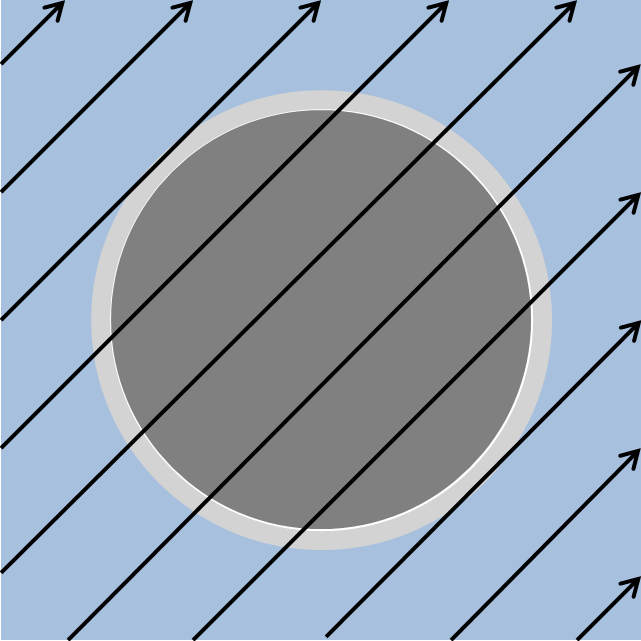
\includegraphics[width=\linewidth]{figures/pin_2.PNG}
		\caption{}
		\label{fig:track-laydown-b}
	\end{subfigure}
	\begin{subfigure}{0.3\textwidth}
		\centering
		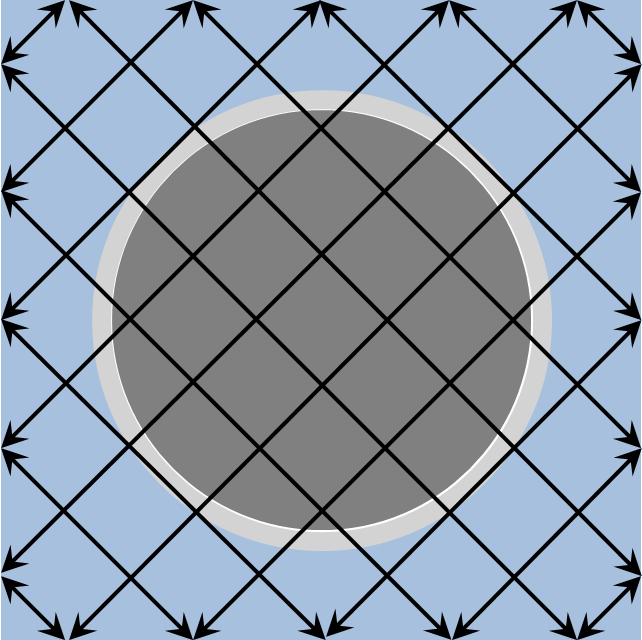
\includegraphics[width=\linewidth]{figures/pin_3.PNG}
		\caption{}
		\label{fig:track-laydown-c}
	\end{subfigure}
	\caption[]{A description of the track laydown process. The geometry (a) is shown followed by the track laydown (b) for one particular direction. Finally the entire track laydown for 4 azimuthal angles is shown (c) with arrows showing that each track is traversed both forward and backward. Note that the track laydowns shown here are significantly coarser than usual track laydowns for illustration purposes.}
	\label{fig:track-laydown}
\end{figure}

Across each track crossing a given constant cross-section source region, the variation of angular flux follows Eq.~\ref{eqn:angular-flux-var}. Therefore, each track is discretized into \textit{segments}, in which each segment is the portion of the track that crosses a particular source region. Across the entire length of each segment Eq.~\ref{eqn:angular-flux-var} applies. An illustration of the segmentation process for the simple pin-cell geometry is shown in Figure~\ref{fig:segmentation}. The presented track, with the geometry drawn along its direction of travel is discretized into segments by material region. For simplicity, this illustration does not discretize the geometry further than material boundaries. A real segmentation process would discretize segments over the domain shown in Figure~\ref{fig:pin-discretization-b}. This process would treat all tracks shown in the track laydown (eg. Figure~\ref{fig:track-laydown}) in a similar manner.

\begin{figure}[h!]
	\centering
	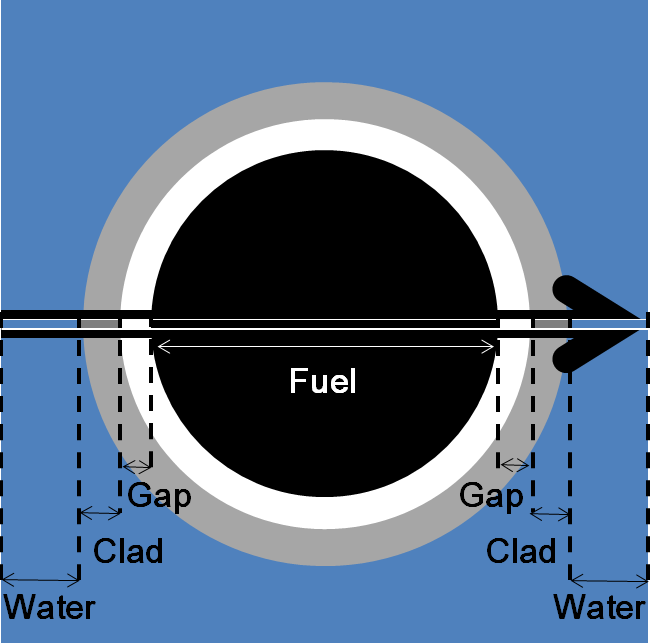
\includegraphics[width=0.6\linewidth]{figures/segmentation.PNG}
	\caption[]{The segmentation of a track horizontally traversing a pin-cell domain with coarse source discretization wherein the boundaries of source regions are no finer than their material region. The formed segments are colored by material region. For illustration purposes, the geometry is not shown to scale.}
	\label{fig:segmentation}
\end{figure}

All of these images showed track laydown and segmentation in just the radial plane, but the same methodology applies for dealing with full three dimensional geometries. Now that tracks have been segmented, a system of equations can be formed governing the variation of angular flux thorough each region as presented in Eq.~\ref{eqn:angular-flux-var}. However, this has a dependence on the incoming angular flux. For segments originating in the bulk of the geometry, continuity of angular flux is naturally enforced. The outgoing flux of the preceding segment in the track provides the incoming flux of the segment. Specifically, the position-dependent angular flux $\psi_{p,g}^{t,\varsigma}(\mathbf{r})$ in group $g$ along track $t$ and segment $\varsigma$ can be expressed as the angular flux of the preceding segment $\varsigma-1$ at the interface point $\mathbf{r_{\textbf{int}}}$ where the segments meet as
\begin{dmath}
	\psi_{p,g}^{t,\varsigma}(\mathbf{r_{\textbf{int}}}) = \psi_{p,g}^{t,\varsigma-1}(\mathbf{r_{\textbf{int}}}).
\end{dmath}
Defining the angular flux along a segment in terms of distance traveled along the segment rather than position, this can equivalently be written as
\begin{dmath}
	\psi_g^{t,\varsigma}(0) = \psi_g^{t,\varsigma-1}(\ell_{t,\varsigma-1})
	\label{eqn:angular_flux_boundary}
\end{dmath}
where $\ell_{t,\varsigma}$ refers to the length of segment $\varsigma$ along track $t$. For angular fluxes originating at the geometry boundary, the boundary condition provides the relationship for the angular flux. For vacuum boundary conditions, it is assumed that there is no impinging angular flux, so the incoming angular flux is simply taken to be zero at the boundary. 

For reflective boundary conditions, the incoming angular flux is equal to the outgoing angular flux of the reflected angle. This requires that a track be present with the correct reflecting angle, meeting at precisely the same point on the boundary. During track laydown, this is enforced. If only vacuum boundary conditions were present, this restriction on track laydown would not be necessary. Similar treatments are possible for periodic and rotational boundary conditions if allowed by the track laydown.  A more complete discussion of track laydown is given in Chapter~\ref{chap:track-laydown}. For instance, the conditions required to link tracks at geometric boundaries will be discussed at length.

Precise definitions are needed in order to discuss the relation of these tracks to the \ac{MOC} equations. Tracks are defined to originate at one boundary and stretch across the geometry until they terminate at another boundary. The segments of a track are ordered in the direction of the track so that only the first segment is affected by a boundary condition. Track $t$ is defined to have $S(t)$ segments. For vacuum boundaries,
\begin{dmath}
	\psi_g^{t,1}(0) = 0
\end{dmath}
For boundary conditions (such as reflective, periodic, and rotational) that connect with another track, the function $C$ is defined which defines the linking track. For instance, the incoming angular flux of track $t$ would connect with the outgoing angular flux of track $C(t)$ as
\begin{dmath}
	\psi_g^{t,1}(0) = \psi_g^{C(t),S(C(t))}(\ell_{C(t),S(C(t))})
	\label{eqn:linking-bc}
\end{dmath}

With the angular and spatial discretization from the track laydown, the angular flux relationship along a characteristic path given in Eq.~\ref{eqn:angular-flux-var} can be presented in terms of the discretized track segments in Eq.~\ref{eqn:angular-flux-var-disc} where the function $R$ yields the region traversed by track $t$ and segment $\varsigma$. 
\begin{dmath}
	\psi_g^{t,\varsigma}(s) = \psi^{t,\varsigma}_g(0) + \left( \frac{q^0_{R(t,\varsigma),g}}{\Sigma_{t}^{i,g}} - \psi_g^{t,\varsigma}(0) \right) F_1\left(\Sigma_{t}^{R(t,\varsigma),g} s \right)
	\label{eqn:angular-flux-var-disc}
\end{dmath}
Still, these equations only determine the behavior of the neutron flux along a particular track. To determine the behavior of the neutron flux throughout the geometry, an infinite number of tracks would be required so that every point in the geometry lies along one of the tracks. Therefore, an approximation is invoked in which all points within the geometry are characterized by the nearest track. Therefore each track represents a volume formed by the product of its length and the perpendicular distances to tracks of the same direction. Those perpendicular lengths form the track cross-sectional area as illustrated in Figure~\ref{fig:track-cross-section}. This illustration just shows the radial view of the tracks. However, in three dimensions, axial distances also exist between tracks so that the track cross-sectional area does indeed represent an area rather than a distance.
\begin{figure}[h!]
	\centering
	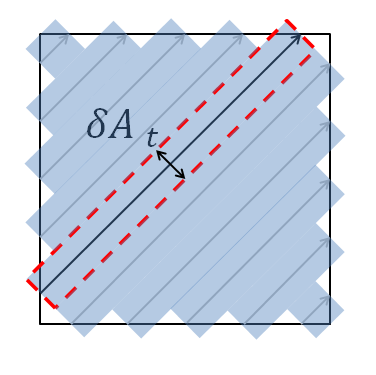
\includegraphics[width=0.6\linewidth]{figures/track-cross-sectional-area.PNG}
	\caption[]{An illustration of the spatial volume represented by each track as the product of track length and track cross-sectional area $\delta A_t$. The volume represented by each track is shaded in blue.}
	\label{fig:track-cross-section}
\end{figure}
With a fine track laydown where the distance between tracks becomes small, the approximation error of assuming points within the geometry are characterized by the nearest track also becomes small. 

However, the neutron transport equation has an angular dependence in addition to a spatial dependence. Therefore, fully resolving the angular dependence would require a track at every direction, again leading to an infinite number of tracks. Similar to the approximation invoked to cover the entire geometric space, the behavior of the neutron flux at each direction is characterized by the track with the most similar direction. This leads to each track $t$ having an angular weight $\alpha_t$ relating to the width of the angular space represented by the track. Therefore the overall weight of the track $w_t$ is calculated as the product of track cross-sectional area and angular weight as given in Eq.~\ref{eqn:weight-def}.
\begin{equation}
w_{t} = \delta A_{t} \alpha_t
\label{eqn:weight-def}
\end{equation}
With each track now representing a portion of the spatial and angular domain, Eq.~\ref{eqn:avg-flux-theory} can be transformed to reflect the track discretization in Eq.~\ref{eqn:average-flux-disc}, yielding a closed-form relationship to calculate the scalar flux.
\begin{dmath}
	\overline{\phi_{i,g}} = \frac{1}{V_i} \sum_{(t,\varsigma) \in V_i} w_{t} \int_{0}^{\ell_{t,\varsigma}} ds \, \psi^{t,\varsigma}_g(s)
	\label{eqn:average-flux-disc}
\end{dmath}
Combining Eq.~\ref{eqn:average-flux-disc} with Eq.~\ref{eqn:angular-flux-var-disc}, the scalar flux can be calculated using the relationship in Eq.~\ref{eqn:average-flux}. A proof is given in Appendix~\ref{deriv:avg-flux} for the interested reader.
\begin{dmath}
	\overline{\phi_{i,g}} = \frac{q^0_{i,g}}{\Sigma_{t}^{i,g}} + \frac{1}{\Sigma_{t}^{i,g} V_i} \sum_{(t,\varsigma) \in V_i} w_{t} \Delta \psi_g^{t,\varsigma}
	\label{eqn:average-flux}
\end{dmath}
The difference in angular flux $\Delta \psi_g^{t,\varsigma}$ is equal to $\psi_g^{t,\varsigma}(0) - \psi_g^{t,\varsigma}(\ell_{t,\varsigma})$. The calculated fluxes can then be used to construct the neutron sources $q^0_{i,g}$ for each region $i$ and each energy group $g$ with the relationship in Eq.~\ref{eqn:source-discr}.


\section{Solving the MOC System of Equations}
\label{sec:moc-solve}

In the previous section Eq.~\ref{eqn:angular-flux-var-disc} and Eq.~\ref{eqn:average-flux} provided ways to calculate the angular fluxes and scalar fluxes, respectively. The source can be computed from the scalar fluxes with Eq.~\ref{eqn:source-discr}. This forms a system of equations that can be solved to determine the neutron distribution inside a nuclear reactor core. Normally, the solution of the \ac{MOC} equations is presented in terms of a physics perspective, following neutrons along trajectories, and repeatedly solving for the neutron source. Physical intuition usually guides this discussion.

The discussion presented here will be more broad. Instead of solely focusing on physics, the problem will be cast as a set of matrix equations that could theoretically be solved with common linear algebra packages. However, this discussion will show that blindly solving the system of equations with a general linear algebra package is computationally infeasible since it loses sight of inherent structure the physics-based approach naturally captures.

The system of equations to be solved is formed by Eq.~\ref{eqn:source-discr}, Eq.~\ref{eqn:angular-flux-var-disc}, and Eq.~\ref{eqn:average-flux}. Turning Eq.~\ref{eqn:source-discr} into matrix form, a fission matrix $F$ and a scattering matrix $S$ are defined such that
\begin{equation}
\mathbf{q} = \frac{1}{k} F \boldsymbol{\phi} + S \boldsymbol{\phi}
\label{eqn:matrix-source-calc}
\end{equation}
where $\mathbf{q}$ is a vector of size $M$ containing all neutron sources and $\boldsymbol{\phi}$ is a vector of size $M$ containing all scalar fluxes. Since there must be a neutron source and scalar flux for every source region and every energy group, $M = L G$ where $L$ is the number of source regions and $G$ is the number of groups. The scalar fluxes $\boldsymbol{\phi}$ as well as the sources $\mathbf{q}$ are ordered such that they are contiguous in group with the index calculated as $i G + g$. In the context of this discussion, elements relating to region quantities are indexed by source region $i$ and group $g$, yielding the following definitions for the fission matrix $F$ and scattering matrix $S$ as
\begin{eqnarray}
F_{\left(i, g\right), \, \left(i, g'\right)} = \frac{1}{4\pi} \chi_{i,g} \nu \Sigma_f^{i,g'}
\label{eqn:fission-matrix}
\end{eqnarray}
and
\begin{eqnarray}
S_{\left(i, g\right), \, \left(i, g'\right)} = \frac{1}{4\pi} \Sigma_s^{i,g' \rightarrow g}
\label{eqn:scattering-matrix}
\end{eqnarray}
where all other unspecified matrix elements are zero. Both of these matrices are of size $M \times M$ and sparse since there are no inter-regional terms.

The relationship in Eq.~\ref{eqn:angular-flux-var-disc} can be rearranged to form the relationship in Eq.~\ref{eqn:re-angular-flux-var-disc}. This form is much easier to work with in the translation to matrix definitions.
\begin{equation}
 \psi^{t,\varsigma}_g(0) \left(\frac{F_1\left(\Sigma_{t}^{i,g} s \right) - 1}{F_1\left(\Sigma_{t}^{i,g} s \right)}\right) + \psi_g^{t,\varsigma}(s) \left(\frac{1}{F_1\left(\Sigma_{t}^{i,g} s \right)}\right) = \frac{q^0_{i,g}}{\Sigma_{t}^{i,g}}
\label{eqn:re-angular-flux-var-disc}
\end{equation}
This relationship can be turned into matrix form by defining an angular flux vector $\boldsymbol{\psi}$ that contains all outgoing angular fluxes. This is represented in Eq.~\ref{eqn:matrix-attn} by an angular flux transport matrix $T$ defining relationships between angular fluxes, a source selection matrix $H$ which selects the source of the region being traversed, and a diagonal matrix $D$ containing the total cross-sections which scale the source appropriately to match the relationship in Eq.~\ref{eqn:re-angular-flux-var-disc}.
\begin{equation}
T \boldsymbol{\psi} = H D^{-1} \mathbf{q}
\label{eqn:matrix-attn}
\end{equation}
The number of angular fluxes is $N = \beta L G$ where $\beta$ is the average number of track crossings per source region. Since there must be a significant number of track crossings per region for convergence we expect $N >> M$. $T$ is size $N \times N$ as it defines relationships between angular fluxes, the size of $H$ is $N \times M$ since for each angular flux pair it must pick out the appropriate source region, and the size of $D$ is $M \times M$ since it relates only to the source regions. The elements relating to angular flux quantities are indexed by track $t$, segment $\varsigma$, and group $g$. The source selection matrix $H$ can therefore be defined as
\begin{equation}
H_{\left(t,\varsigma,g\right), \, \left(R(t,\varsigma), g\right)} = 1.
\label{eqn:source-selection-matrix}
\end{equation}
This matrix therefore, has only one non-zero value per row, indicating which region is being traversed, relating track-based quantities such as angular fluxes to region based quantities such as the scalar fluxes. Its transpose similarly relates the regions to the tracks traversing the region. The matrix $H^T H$ is a $M \times M$ diagonal matrix with each diagonal element representing the number of tracks that traverse the region multiplied by the number of groups. Since it is diagonal, it is easily invertible, which will be important in the later discussion.
The diagonal matrix $D$ containing the total cross-sections is defined by
\begin{equation}
D_{\left(i, g\right), \, \left(i, g\right)} = \Sigma_t^{i,g}.
\label{eqn:total-xs-matrix}
\end{equation}
The angular flux transport matrix $T$ is defined by
\begin{equation}
T_{\left(t,\varsigma,g\right), \, \left(t, \varsigma, g\right)} = \frac{1}{F_1\left(\Sigma_{t}^{R(t,\varsigma),g} \ell_{t,\varsigma}\right)}
\label{eqn:angular-flux-transport-matrix-1}
\end{equation}
and
\begin{equation}
T_{\left(t,\varsigma,g\right), \, \left(t, \varsigma-1, g\right)} = \frac{F_1\left(\Sigma_{t}^{R(t,\varsigma),g} \ell_{t,\varsigma}\right) - 1}{F_1\left(\Sigma_{t}^{R(t,\varsigma),g} \ell_{t,\varsigma}\right)}.
\label{eqn:angular-flux-transport-matrix-2}
\end{equation}
Again, all non-specified quantities are zero.

Lastly, Eq.~\ref{eqn:average-flux} describes how the scalar flux can is calculated in terms of both a weighted sum of angular fluxes and the neutron source. Specifically, an angular flux weighting matrix $W$ of size $M \times N$ is defined such that
\begin{equation}
\boldsymbol{\phi} = D^{-1}\mathbf{q} + D^{-1} W \boldsymbol{\psi}.
\label{eqn:matrix-flux-calc}
\end{equation}
In order to expose its structure, $W$ is expressed as a multiplication of matrices
\begin{equation}
W = V^{-1} H^T \tilde{W}
\end{equation}
where the volume matrix $V$ is a $M \times M$ diagonal matrix containing region volumes as
\begin{equation}
V_{\left(i, g\right), \, \left(i, g\right)} = V_i
\end{equation}
and $\tilde{W}$ is an $N \times N$ matrix defined by
\begin{equation}
\tilde{W}_{\left(t,\varsigma,g\right), \, \left(t, \varsigma, g\right)} = -w_{t}
\end{equation}
and
\begin{equation}
\tilde{W}_{\left(t,\varsigma,g\right), \, \left(t, \varsigma-1, g\right)} = w_{t}
\end{equation}
with all other elements being zero. Now that all matrix elements have been defined, the transport equation can be written as a matrix eigenvalue problem. Combining Eq.~\ref{eqn:matrix-source-calc} and Eq.~\ref{eqn:matrix-flux-calc} yields
\begin{equation}
\boldsymbol{\phi} = D^{-1} \left(\frac{1}{k} F + S \right) \boldsymbol{\phi} + D^{-1} W \boldsymbol{\psi}
\end{equation}
which combined with Eq.~\ref{eqn:matrix-attn} yields
\begin{equation}
\boldsymbol{\phi} = D^{-1}\left( I + W T^{-1} H D^{-1}\right) \left(\frac{1}{k} F + S \right) \boldsymbol{\phi}
\label{eqn:moc-matrix-form}
\end{equation}
where $I$ is the identity matrix of dimension $M \times M$. This relationship can be further simplified by defining a matrix $J$ such that
\begin{equation}
J = D^{-1}\left( I + W T^{-1} H D^{-1}\right)
\end{equation}
leading to the expression
\begin{equation}
\boldsymbol{\phi} = J \left(\frac{1}{k} F + S \right) \boldsymbol{\phi}
\label{eq:transport-simplified}
\end{equation}
This results in the generalized eigenvalue equation given in Eq.~\ref{eqn:gen-eig}
\begin{equation}
A \boldsymbol{\phi} = k B \boldsymbol{\phi}
\label{eqn:gen-eig}
\end{equation}
where
\begin{equation}
A = JF
\end{equation}
and
\begin{equation}
B = I - JS.
\end{equation}
This can of course be turned into a regular eigenvalue problem by explicitly taking the inverse as
\begin{equation}
B^{-1}A \boldsymbol{\phi} = k \boldsymbol{\phi}.
\label{eqn:eig}
\end{equation}
At this point, the matrix $B^{-1}A$ could be explicitly calculated and then input into any standard eigenvalue solver. However, taking matrix inverses is very computationally intense, especially due to the internal structure of $A$ and $B$. Specifically, since $J$ involves the inverse of $T$, even the explicit computation of its elements is infeasible. Therefore, doing this would be very unwise. Even if a generalized eigenvalue solver is available capable of solving equations of the form given in Eq.~\ref{eqn:gen-eig}, the problem would still rely on computing explicit components of $J$. Even though the steady-state neutron transport equation is an eigenvalue problem defined in terms of the angular fluxes, they only enter the equation implicitly with the inversion of $T$. 

%Moreover, the reaction rates of interest are defined in terms of the scalar fluxes. From angular fluxes, it is simple to calculate the scalar fluxes. This structure is an indication that explicitly solving for the full vector of angular fluxes is unnecessary.

Therefore, instead of using a common eigenvalue solution technique, a variation of fixed point iteration termed \textit{source iteration} is chosen to solve the system. In this procedure, the relationship in Eq.~\ref{eqn:moc-matrix-form} is used with the right hand side of the equation lagged as
\begin{equation}
\boldsymbol{\phi}_{n+1} = D^{-1}\left( I + W T^{-1} H D^{-1}\right) \left(\frac{1}{k_n} F + S \right) \boldsymbol{\phi}_n
\end{equation}
where the subscript $n$ indicates iteration number. Mechanically, the process iterates over estimations of the neutron source, calculating the corresponding fluxes. First, an initial flux distribution is guessed along with a value for the eigenvalue $k$. At the start of each iteration, the source distribution $\mathbf{q}$ is calculated using Eq.~\ref{eqn:matrix-source-calc} from the current guess of scalar fluxes $\boldsymbol{\phi}$ and eigenvalue $k$. Then, during the \textit{transport sweep}, new angular fluxes are computed as
\begin{equation}
\boldsymbol{\psi} = T^{-1} H D^{-1} \mathbf{q}.
\end{equation}
First, the computation of $HD^{-1}\mathbf{q}$ is trivial since $H$ is just the source selection matrix and $D$ is diagonal. Physically, this just relates to picking out the source region being traversed and calculating the source divided by the total cross-section.

Due to the simple structure of $T$, solving its implicit inversion is rather simple. $T$ has just one element on the diagonal and one off-diagonal element per row. Note that the angular fluxes are only related to their associated connecting angular flux. For some boundary conditions (e.g. reflective), the connecting angular flux might be from another track. This could cause the inversion to be somewhat difficult. If all boundaries have this characteristic, all the angular fluxes within a cycle of connecting tracks would be dependent on each other.

To alleviate this issue, the angular fluxes at boundaries are approximated by the calculated angular flux at the boundary from the previous iteration. Specifically, the relationship in Eq.~\ref{eqn:angular_flux_boundary} relating connecting angular fluxes at the start of a track is approximated by
\begin{dmath}
	\psi_g^{t,1}(0) = \widetilde{\psi}_g^{C(t),S(C(t))}(\ell_{C(t),S(C(t))})
\end{dmath}
where $\widetilde{\psi}$ represents the calculated angular fluxes from the previous iteration so that $\widetilde{\psi}_g^{C(t),S(C(t))}$ is the angular flux of the connecting track from the previous iteration. This transformation allows the inversion of $T$ to be calculated using an altered matrix $\tilde{T}$ which lacks dependency between different tracks, then adding the contribution of the previous iteration angular fluxes, if applicable. The structure of $\tilde{T}$ is block-diagonal and within each block the matrix is upper triangular. Physically this means that all tracks can be calculated independently of each other during an iteration. For each track, the angular fluxes can be solved sequentially by segment. This is where the \textit{transport sweep} owes its name as the algorithm simply sweeps over segments. Since each row has at most two elements, very little calculation is required for each angular flux. 

During this process, it is noted that only the boundary angular fluxes along with the neutron source are needed to determine all angular fluxes. Therefore, non-boundary angular fluxes are computed on-the-fly. Furthermore, the elements of $T$ are re-computed on-the-fly. Since the computation of the scalar fluxes $\boldsymbol{\phi}$ relies on a weighted sum of the full angular flux vector $\boldsymbol{\psi}$, once an angular flux is computed its contribution to the scalar fluxes is tallied before it is discarded.

After the transport sweep, the source is added to the scalar flux tally, consistent with Eq.~\ref{eqn:matrix-flux-calc}, to produce a new estimate of the scalar fluxes $\boldsymbol{\phi}$. To form a new estimate of $k$, note that
\begin{equation}
T \boldsymbol{\psi} = \frac{1}{k} H D^{-1} F \boldsymbol{\phi} + H D^{-1} S \boldsymbol{\phi}
\end{equation}
which then is re-arranged and multiplied with a vector of ones $\mathbb{1}_M$ of length $M$ as
\begin{equation}
\mathbb{1}_M^T D H_{\text{left}}^{-1} T \boldsymbol{\psi}  = \frac{1}{k} \mathbb{1}_M^T  F \boldsymbol{\phi} + \mathbb{1}_M^T  S \boldsymbol{\phi}.
\end{equation}
Since $H$ is rectangular, it cannot be simply inverted. But since it is of full rank, $H^T H$ can be inverted. From the previous discussion of $H$, recall that $H^T H$ is diagonal so its inversion is simple. Therefore the left inverse $H_{\text{left}}^{-1}$ of matrix $H$ is defined to be
\begin{equation}
H_{\text{left}}^{-1} = \left(H^T H\right)^{-1} H^T.
\end{equation}
This allows the eigenvalue $k$ to be computed as
\begin{equation}
k = \frac{\mathbb{1}_M^T F \boldsymbol{\phi}}{\mathbb{1}_M^T  D H_{\text{left}}^{-1} T \boldsymbol{\psi} - \mathbb{1}_M^T S \boldsymbol{\phi}}.
\end{equation}
Combining Eq.~\ref{eqn:matrix-attn} and Eq.~\ref{eqn:matrix-flux-calc}, note that
\begin{equation}
D H_{\text{left}}^{-1} T \boldsymbol{\psi} = D \boldsymbol{\phi} - W \boldsymbol{\psi}
\end{equation}
and therefore
\begin{equation}
k = \frac{\mathbb{1}_M^T F \boldsymbol{\phi}}{\mathbb{1}_M^T \left(D - S \right) \boldsymbol{\phi} - \mathbb{1}_M^T W \boldsymbol{\psi}}.
\end{equation}
where $\mathbb{1}_M^T F \boldsymbol{\phi}$ refers to the fission rate, $\mathbb{1}_M^T \left(D - S \right) \boldsymbol{\phi}$ refers to the absorption rate, and $-\mathbb{1}_M^T W \boldsymbol{\psi}$ refers to the leakage rate. Physically, this shows that $k$ is simply a ratio of neutron production to neutron loss terms.

Notice that each source iteration relies on simply taking the inverse of the transport matrix $T$ rather than the full $B$ matrix, which includes the scattering matrix, as would normally be taken during an eigenvalue solver, e.g. power iteration. While this choice does ease the computational burden of each iteration, it also requires many more iterations to converge to the correct solution as each iteration does little work in resolving the angular fluxes as the scattering matrix is not included in the inversion. Physically, this relates to not treating the scattering source as directly coupled to the total neutron source. Therefore, un-accelerated \ac{MOC} is inherently plagued by slow convergence. 

Next, in Chapter~\ref{chap:cmfd}, Course Mesh Finite Difference (CMFD) acceleration is introduced which resolves the issue of slow convergence for source iteration. This allows for the computational burden of each iteration to be eased without giving up anything in terms of convergence rate by iteration.

\newpage
\vfill
\begin{highlightsbox}[frametitle=Highlights]
	\begin{itemize}
		\item The \ac{MOC} transform changes the neutron transport equation from a partial differential equation to an ordinary differential equation along a certain direction.
		\item The geometry is discretized into source regions which have constant cross-sections and a low-order approximation of the neutron source within the region.
		\item Tracks are laid down across the geometry which enable the  \ac{MOC} transform to yield an analytic description of the angular flux variation across each source region.
		\item The angular flux variation along each track provided a weighted contribution to the scalar flux estimate of each traversed source region.
		\item The synthesis of \ac{MOC} equations over each source region form an eigenvalue problem.
		\item The \ac{MOC} eigenvalue problem fundamentally involves all angular fluxes over each source region.
		\item Since the number of angular fluxes is vast, standard eigenvalue solution techniques are abandoned in favor of \textit{source iteration} which takes advantage of fundamental structure of the \ac{MOC} equations.
		\item \textit{Source iteration} allows each \ac{MOC} iteration to be computed far more efficiently in the form of a \textit{transport sweep} but at the cost of slow convergence (if acceleration is absent)
	\end{itemize}
\end{highlightsbox}


%\begin{equation}
%\left(I - JS\right)^{-1} JF \boldsymbol{\phi} = k \boldsymbol{\phi}
%\end{equation}

%\begin{equation}
%A \boldsymbol{\phi} = k \boldsymbol{\phi}
%\end{equation}

%\begin{equation}
%\boldsymbol{\phi}_{n+1} = J \left(\frac{1}{k_n} F + S\right) \boldsymbol{\phi}_n
%\end{equation}

%\begin{equation}
%\boldsymbol{\phi}_{n+1} = J \left(\frac{1}{k} F + S\right) \boldsymbol{\phi}_n
%\end{equation}

%\begin{equation}
%\boldsymbol{\phi}_{n+1} = B \boldsymbol{\phi}_n
%\end{equation}

%\begin{equation}
%B \boldsymbol{\phi} = \lambda \boldsymbol{\phi}
%\end{equation}


%\begin{equation}
%\boldsymbol{\phi} + C \boldsymbol{\phi} = J \left(\frac{1}{k} F + S\right) \boldsymbol{\phi} + C \boldsymbol{\phi}
%\end{equation}

%\begin{equation}
%\left(I + C\right)\boldsymbol{\phi}_{n+1} = J \left(\frac{1}{k_n} F + S\right) \boldsymbol{\phi}_n + C \boldsymbol{\phi}_n
%\end{equation}

%\begin{equation}
%\boldsymbol{\phi}_{n+1} = \left(I + C\right)^{-1} \left[J \left(\frac{1}{k_n} F + S\right) + C\right] \boldsymbol{\phi}_n
%\end{equation}